%\chapter{開発プロセス}
\section{第3サイクル}
第3サイクルは後期が始まった9月25日から10月21日に行われた外部講師によるリモートレビューまでとした。本サイクルでは、第2サイクルで見つかった大きな課題の一つである写真を撮る行為にもっとワクワクするような付加価値を加えなければならないこと、そして観光情報をより魅力的に紹介することを課題として活動を進めた。\\
まず我々は、後期が始まって最初のプロジェクト学習で前期を振り返り、もう一度課題を見直した。そして観光情報の表示の仕方について話し合った時、「札幌でしかできない50のこと」と言うネットの記事があるということを知り、それを参考にして木古内で「できること」に着目した情報の紹介する形式にすることを決定した。また、それと同時に「アプリからトランプを作れたら面白いのでは」と言う意見が出たため、そのアイディアを膨らませて撮った写真を利用してカルタという「もの」にする機能を作ることも決定した。この時、リモートレビューまでには出来る範囲までは実装を行おうということで、木古内で「できること」に着目した情報紹介の機能から実装を進めた。具体的に修正した内容を表5.3に、実装はこの時マージが完了していなかったので、完成した画面イメージを図5.3(a)に示す。\\本サイクルではより魅力的な観光情報を表示できるようになったこと、また写真を撮るモチベーションを上げるものとして実際にカルタという「もの」にできるという解決策になった。しかし、カルタは50枚を超える紙を印刷するのは手間がかかるという課題が残った。

\begin{table}[htb]
\centering
\addtocounter{table}{+0}
\caption{第2サイクルから第3サイクルへの変化}
  \begin{tabular}{|l|l|} \hline
    改正前&改正後  \\ \hline 
    カテゴリごとに写真の一覧を表示 & \parbox{20zw}{写真と同時に紹介文を加えることで木古内で「できること」に着目した情報を表示} \\  \hline
    詳細情報を表示してからマップに遷移 &\parbox{20zw}{マップ画面と同時に詳細情報や写真を表示}\\ \hline
    「フォトストーリ―」という機能でアプリ内で写真を振り返る & \parbox{20zw}{カルタという「もの」にして思い出を残す}\\ \hline
  \end{tabular} 
\end{table}

\begin{figure}[htbp]
  \begin{center}
    \begin{tabular}{c}

      % 1
      \begin{minipage}{0.33\hsize}
        \begin{center}
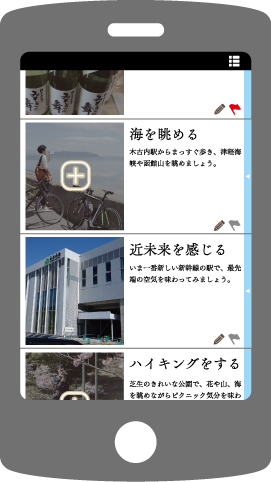
\includegraphics[width=4cm, bb=0 0 320 552]{画面案1.png}
          \hspace{1cm} [1]観光スポットの紹介
        \end{center}
      \end{minipage}

      % 2
      \begin{minipage}{0.33\hsize}
        \begin{center}
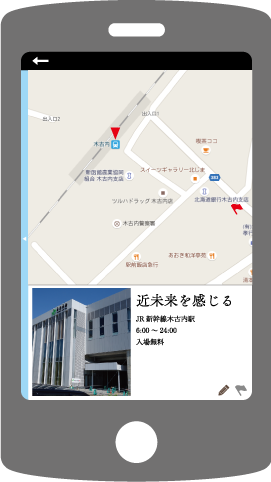
\includegraphics[width=4cm, bb=0 0 321 547]{画面案2.png}
          \hspace{1cm} [2]詳細情報の表示
        \end{center}
      \end{minipage}

      % 3
      \begin{minipage}{0.33\hsize}
        \begin{center}
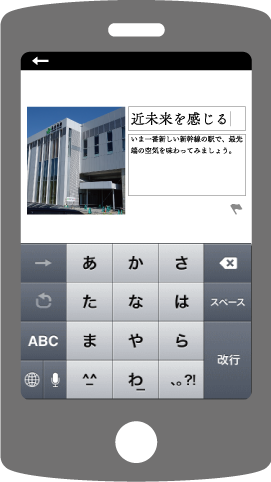
\includegraphics[width=4cm, bb=0 0 320 548]{画面案3.png}
          \hspace{1cm} [3]紹介文の編集
        \end{center}
      \end{minipage}

    \end{tabular}
    \caption{(a)第3サイクルの完成画面イメージ}
    \label{fig:lena}
  \end{center}
\end{figure}

\begin{description}
 \item[フォトストーリーの説明]\mbox{}
 \begin{enumerate}
 \item フォトストーリーを使用することでどのような紀行が出来上がるのかのサンプル動画を見る。この動画にはフォトストーリーの操作説明及び木古内町の魅力が内容として含まれているため、操作方法だけでなく木古内の魅力も知ることができる。
  \item 観光中に撮影した写真をアプリ内に保存。
 \item 撮影した写真の一覧が表示され、ユーザが写真を任意のカテゴリ別に分けることができる。
 \item 加工ボタンを押すとユーザが撮影した写真と移動した経路を表示したマップが紀行として画面に表示される。
 \item フォトストーリーを使用してユーザの思い出話によるコミュニケーションが促進される。
\end{enumerate}
\item[フォトストーリーへのレビュー内容]\mbox{}
 \begin{itemize}
 \item 木古内町の歴史に関する情報を表示する機能が欲しい
 \item 図5.2(b)に対して、1 つの画面に写真が2 枚もあると分かりにくい
 \item 写真を撮りたくなるトリガーがないため、フォトストーリの存在が危うい
 \item 時系列での説明をされると聞いている側は辛くなってしまう。2,3枚ほどのダイジェストの方が良い。
 \item フォトストーリーを実装するのであれば、誰が写真を撮るのかを考えてUI設計を行うこと。スマートフォンに使い慣れた若い人と大人と子供ではそれぞれUIが違ってくる。
 \item 案内だけに留まらずに思い出に着眼したことは良い。今後の掘り下げ方で何倍にも良いものになる可能性がある。
 \end{itemize}
\end{description}

\begin{figure}[htbp]
  \begin{center}
    \begin{tabular}{c}

      % 1
      \begin{minipage}{0.33\hsize}
        \begin{center}
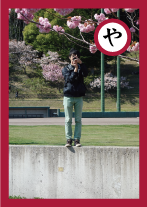
\includegraphics[width=4cm, bb=0 0 320 552]{かるた案1.png}
        \end{center}
      \end{minipage}

      % 2
      \begin{minipage}{0.33\hsize}
        \begin{center}
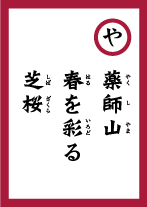
\includegraphics[width=4cm, bb=0 0 321 547]{かるた案5.png}
        \end{center}
      \end{minipage}

      % 3
      \begin{minipage}{0.33\hsize}
        \begin{center}
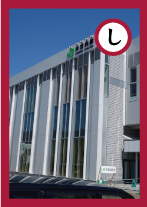
\includegraphics[width=4cm, bb=0 0 320 548]{かるた案4.png}
        \end{center}
      \end{minipage}

    \end{tabular}
  \end{center}
\addtocounter{figure}{+0}
 \caption{(b)カルタの完成サンプル}
\end{figure}


\bunseki{山川拓也}